% ============================================================
% ESTRATÉGIA EMPÍRICA
% ============================================================

% -------------------------------------------------------
\section{Estratégia Empírica}
% -------------------------------------------------------

\begin{frame}[plain]
    \vfill
    \centering
    \begin{beamercolorbox}[sep=12pt,center,shadow=false,rounded=true]{title}
        {\Large\bfseries Estratégia Empírica}\\[6pt]
        {\normalsize Dados, identificação e o experimento natural de Brasília}
    \end{beamercolorbox}
    \vfill
\end{frame}

\begin{frame}{Dados}
    \begin{columns}[T]
        \begin{column}{0.48\textwidth}
            \textbf{Migração}
            \begin{itemize}
                \item Censos decenais: 1940--2000.
                \item \textit{Estoque de pessoas em cada estado}, desagregado por estado de nascimento.
                \item 21 UFs destino $\times$ 20 UFs origem $\times$ 7 anos $= 2.940$ observações bilaterais.
            \end{itemize}
        \end{column}
        \begin{column}{0.48\textwidth}
            \textbf{Comércio}
            \begin{itemize}
                \item Anuários estatísticos: 1942--1949, 1959--1974, 1985, 1998--1999.
                \item \textit{Valor anual de importações} por estado, desagregado por estado de origem.
                \item 21 UFs destino $\times$ 20 UFs origem $\times$ 27 anos $= 2.940$ observações bilaterais.
            \end{itemize}
        \end{column}
    \end{columns}

    \vspace{0.4cm}

    \textbf{Malha rodoviária}
    \begin{itemize}
        \item Mapas georreferenciados do DNIT: 1960--2000 (rodovias federais pavimentadas).
        \item Redes de 1940 e 1950 reconstruídas por fontes históricas.
        \item \textit{Tempo de viagem} entre centroides estaduais calculado por algoritmo \textit{fast marching}.
    \end{itemize}
\end{frame}

\begin{frame}{Modelo de gravidade -- Forma genérica}
    Para estimar a resposta de migração e de comércio às mudanças no tempo de viagem rodoviário, os autores estimam uma \textbf{equação de gravidade}:

    \begin{equation}\label{eq:gravity}
        M_{odt} = \gamma_{ot} + \gamma_{dt} + \gamma_{od}
                  + \beta \log \text{tempo de viagem}_{odt} + \varepsilon_{odt}
    \end{equation}

    \vspace{0.15cm}

    \begin{itemize}
        \item $M_{odt}$: fluxo bilateral de migração \textit{ou} comércio (origem $o$, destino $d$, ano $t$).
        \item $\gamma_{ot}$, $\gamma_{dt}$: efeitos fixos de origem-ano e destino-ano.
        \item $\gamma_{od}$: efeito fixo de par -- controla por heterogeneidades invariante no tempo (distância, proximidade cultural, redes históricas).
        \item $\beta$: \textit{elasticidade} de migração (ou comércio) ao tempo de viagem (esperado $\beta < 0$).
    \end{itemize}
\end{frame}

\begin{frame}{Identificação -- O problema}
    \begin{block}{Problema de endogeneidade}
        A expansão rodoviária entre dois estados pode ser correlacionada com um choque econômico naquele par. Exemplo: um choque negativo leva o governo a investir em infraestrutura \textit{e} desestimula migração/comércio simultaneamente $\Rightarrow$ viés positivo em $\hat\beta$.
    \end{block}

    \vspace{0.4cm}

    \begin{block}{Solução: experimento natural}
        Em 1960, o Brasil construiu \textbf{Brasília} e inaugurou uma rede de rodovias radiais conectando a nova capital às demais capitais estaduais nas oito direções cardeais e intercardeais. Essa rede foi determinada pela \textbf{localização da capital}, não por demanda por comércio ou migração entre pares de estados.
    \end{block}
\end{frame}

\begin{frame}{Identificação -- O instrumento MST}
    \textbf{Minimum Spanning Tree (MST):} rede rodoviária predita, construída em quatro etapas:

    \begin{enumerate}
        \item Sobrepõe o mapa do Brasil a um círculo centrado em Brasília.
        \item Divide o círculo em \textbf{8 fatias} de tamanho igual (direções cardeais e intercardeais).
        \item Dentro de cada fatia, calcula o \textbf{menor caminho} de Brasília até as capitais estaduais contidas nela.
        \item Une os oito caminhos $\Rightarrow$ rede MST.
    \end{enumerate}

    \vspace{0.3cm}

    A rede MST altera o tempo de viagem entre pares de estados $\Rightarrow$ \textbf{instrumento para a rede rodoviária efetiva}.

    \vspace{0.2cm}

    \small\textit{O MST responde à pergunta: ``se o único objetivo fosse conectar Brasília às capitais pelo caminho mais curto, como seria a rede?'' Essa rede predita gera variação no tempo de viagem determinada por geometria e pela localização da capital --- não por demanda econômica --- e é essa variação que identifica $\beta$ de forma causal.}
\end{frame}

\begin{frame}{Identificação -- O instrumento MST}
    \begin{figure}[H]
        \centering
        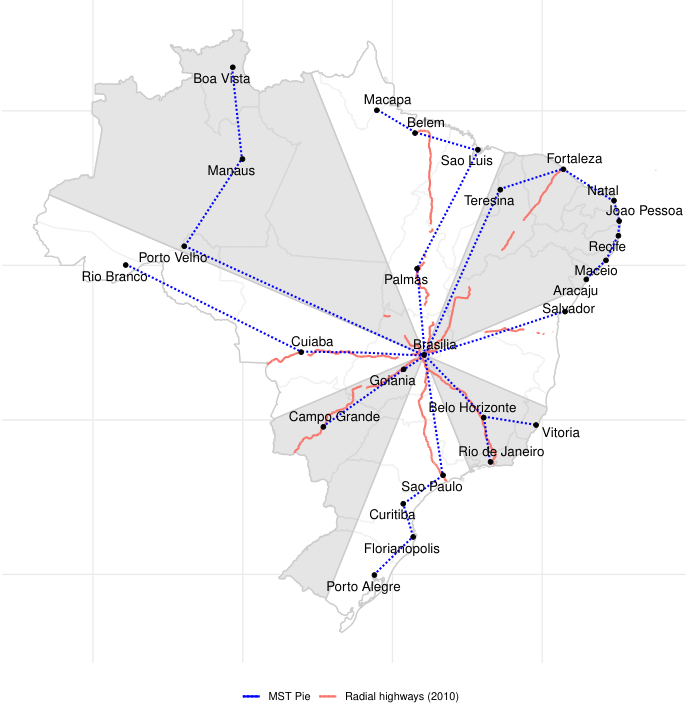
\includegraphics[width=0.4\textwidth]{figures/fig1.png}
        
        \scriptsize{Fonte: Morten e Oliveira (2023).}
    \end{figure}
\end{frame}

\begin{frame}{Análise econométrica -- Especificação com instrumento}
    Para verificar os efeitos ao longo do tempo, os autores estimam:

    \begin{equation}\label{eq:iv}
        \log y_{odt} = \gamma_{ot} + \gamma_{dt} + \gamma_{od}
                      + \alpha_t\;\underbrace{\text{MST-induced Reduction in TT}_{od}}_{\text{redução predita no tempo de viagem}}
                      + v_{odt}
    \end{equation}

    \vspace{0.15cm}

    \begin{itemize}
        \item $y_{odt}$: tempo de viagem real, migração \textit{ou} comércio (origem $o$, destino $d$, ano $t$).
        \item \textbf{Instrumento invariante no tempo:} redução percentual no tempo de viagem predita pela rede MST.
        \item $\alpha_t$ varia por ano $\Rightarrow$ testa \textit{quando} os efeitos se manifestam (pré e pós-Brasília).
        \item Normalizado em relação a 1950 (último ano pré-Brasília); erros clusterizados no par $(o,d)$.
    \end{itemize}
\end{frame}

\begin{frame}{Análise econométrica -- Efeitos ao longo do tempo}
    \begin{columns}[T]
        \begin{column}{0.4\textwidth}
            \vspace{0.7cm}
            \begin{itemize}\small
                \item \textbf{Sem pré-tendências:} coeficiente em 1940 não difere de zero -- sem viés de antecipação.
                \item \textbf{Após 1960:} queda abrupta no tempo de viagem e aumento em migração e comércio.
                \item Coef.\ de 1960: $+0{,}4$ (migração) e $+1{,}4$ (comércio) $\Rightarrow$ diferença de 10 p.p.\ na redução MST-predita implica $+$4\% em migração e $+$14\% em comércio relativo a 1950.
            \end{itemize}
        \end{column}
        \begin{column}{0.6\textwidth}
            \vspace{-.3cm}
            \begin{figure}[H]
                \centering
                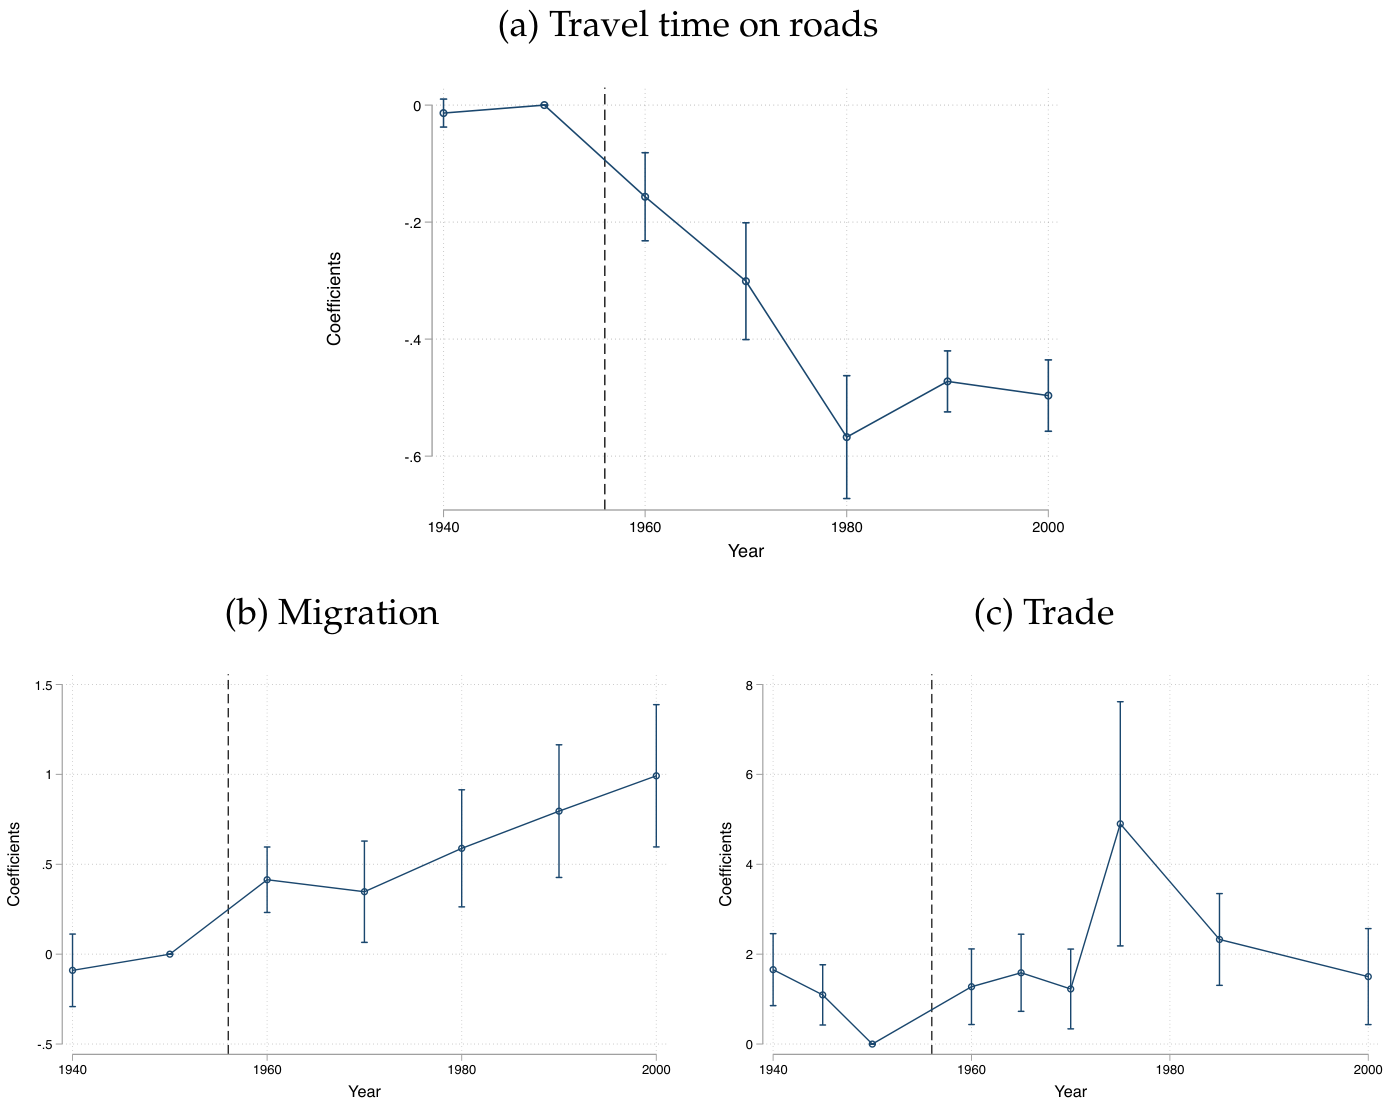
\includegraphics[width=0.85\textwidth]{figures/fig2.png}\\[2pt]
                \scriptsize{Fonte: Morten e Oliveira (2023).}
            \end{figure}
        \end{column}
    \end{columns}
\end{frame}


\begin{frame}{Resultados -- Estradas promovem migração e comércio}
    \begin{center}
        {\small{Tabela 1 - Elasticidades de migração e comércio ao tempo de viagem rodoviário}}
    \end{center}
    \vspace{-0.2cm}
    \resizebox{\textwidth}{!}{%
    \begin{tabular}{lcccccccc}
        \toprule
         & \multicolumn{4}{c}{Migração} & \multicolumn{4}{c}{Comércio} \\
        \cmidrule(lr){2-5}\cmidrule(lr){6-9}
         & (1) & (2) & (3) & (4) & (5) & (6) & (7) & (8) \\
         & MQO & VI & PPML & PPML & MQO & VI & PPML & PPML \\
        \midrule
        Log tempo de viagem em rodovias
            & \textcolor{red}{$-0.332^{***}$} & \textcolor{red}{$-1.753^{***}$} & $-0.560^{***}$ & $-2.123^{***}$
            & \textcolor{red}{$-0.783^{***}$} & \textcolor{red}{$-1.890^{***}$} & $-0.145$ & $-1.963^{***}$ \\
            & $(0.116)$ & $(0.454)$ & $(0.124)$ & $(0.336)$
            & $(0.155)$ & $(0.521)$ & $(0.204)$ & $(0.437)$ \\
        \midrule
        $N$
            & 2.939 & 2.939 & 2.940 & 2.940
            & 7.451 & 7.451 & 8.960 & 8.960 \\
        F-stat
            & 8,180 & 14,910 & & & 25,586 & 13,142 & & \\
        F-stat 1\textordfeminine{} etapa
            & & & 22,086 & & & & 11,217 & \\
        Controle res.\ 1\textordfeminine{} etapa
            & & & Não & Sim & & & Não & Sim \\
        \bottomrule
    \end{tabular}%
    }\\[4pt]
    {\tiny E.P.\ clusterizados no par entre parênteses. Cols.\ (1), (2), (5), (6): MQO/VI, dependente em log. Cols.\ (3)--(4), (7)--(8): PPML. \\ $^*p{<}0{,}1$, $^{**}p{<}0{,}05$, $^{***}p{<}0{,}01$. \\ Fonte: Morten e Oliveira (2023).}
\end{frame}

\begin{frame}{Resultados -- Principais achados}
    \begin{itemize}
        \item \textbf{Estimativas VI superam MQO -- viés de endogeneidade confirmado:}
        \begin{itemize}
            \item Migração: MQO $= -0{,}33$ \textit{vs.}\ VI $= -1{,}75$
            \item Comércio: MQO $= -0{,}78$ \textit{vs.}\ VI $= -1{,}90$
        \end{itemize}
        \item A expansão rodoviária respondeu positivamente a choques negativos $\Rightarrow$ MQO \textbf{subestima} os efeitos das estradas.

        \vspace{0.15cm}

        \item \textbf{PPML com função de controle} (cols.\ 4 e 8) -- robusto a fluxos zero:
        \begin{itemize}
            \item Migração: elasticidade $-2{,}12$ (estatisticamente indistinguível de $-1{,}75$).
            \item Comércio: elasticidade $-1{,}96$ (estatisticamente indistinguível de $-1{,}90$).
        \end{itemize}

        \vspace{0.15cm}

        \item \textbf{Robustez:} excluir pares com Goiás (sede de Brasília) não altera as estimativas -- o efeito não é artificialmente gerado pela nova capital.
    \end{itemize}
\end{frame}